\documentclass{article}

% Paquetes (estilo base de la plantilla de Overleaf)
\usepackage[T1]{fontenc}
\usepackage[spanish,es-tabla,es-noquoting,es-nodecimaldot]{babel}
\usepackage{csquotes}
\usepackage[letterpaper,top=2cm,bottom=2cm,left=3cm,right=3cm,marginparwidth=1.75cm]{geometry}
\usepackage{amsmath}
\usepackage{graphicx}
\usepackage{booktabs}
\usepackage{tabularx}
\usepackage{float}
\usepackage[section]{placeins}
\usepackage[colorlinks=true, allcolors=blue]{hyperref}
\usepackage[backend=biber, style=authoryear]{biblatex}
\addbibresource{references.bib}

\title{Clasificación supervisada de coberturas tras el colapso de la presa de Brumadinho (Minas Gerais, Brasil) con Sentinel-2\\[0.5em]
\large Proyecto final -- Fase 2: preprocesamiento y entrenamiento}
\author{Jose Villarroel, Jose D. Medina, Camila Beltrán y Juan Rodríguez\\Pontificia Universidad Javeriana}
\date{\today}

\begin{document}

\maketitle

\begin{abstract}
Este documento presenta la segunda fase del análisis comparativo de arquitecturas de aprendizaje automático para clasificar coberturas en Brumadinho (Brasil) con una escena Sentinel-2 del 1 de febrero de 2019. Primero se documenta el archivo TSV de entrenamiento: 1640 píxeles, doce bandas y seis clases, extraídos de 88 polígonos. Luego se describen su preprocesamiento y dos formas de entrenamiento con los cinco modelos del enunciado más Random Forest: la pista A entrena con píxeles y se evalúa por píxel y por polígono; la pista B entrena con la mediana de cada polígono más índices espectrales. La prueba actual son 24 polígonos originales; los polígonos añadidos se usan solo para entrenamiento. Sobre la prueba original, definida antes de la ampliación, la regresión logística y la SVM alcanzan una exactitud global de 89{,}4\,\%; es el resultado de referencia de esta fase. Dos polígonos de suelo que los modelos fallaban se retiraron después de esa evaluación; en la prueba actual, sin ellos, ambos modelos llegan a 94{,}7\,\% (Kappa 0{,}935), pero esa cifra puede estar sesgada a favor de los modelos y no demuestra una mejora. Los errores se concentran en suelo expuesto y urbano.
\end{abstract}

\section{Introducción}
En la Fase~1 se definieron el evento de estudio, el área de estudio y la imagen satelital, y se construyó el conjunto de datos de entrenamiento \texttt{training\_dataset.tsv}. Esta segunda fase tiene dos objetivos, según el enunciado del proyecto:
\begin{enumerate}
 \item documentar el archivo TSV de entrenamiento exportado;
 \item entrenar los modelos y reportar sus métricas iniciales de evaluación, como mínimo la matriz de confusión y la exactitud global.
\end{enumerate}
Los modelos se implementaron en Python con scikit-learn \parencite{Pedregosa2011}. La optimización de hiperparámetros, la comparación formal entre arquitecturas y la predicción sobre la imagen completa corresponden a la Fase~3.

Además de las métricas por píxel, esta fase evalúa la unidad de análisis por polígono. Los resultados se reportan con el polígono como unidad de muestreo y de validación, y la ampliación del conjunto de entrenamiento se compara con la versión anterior sobre el mismo test.

\section{Documentación del archivo TSV}

\subsection{Estructura y contenido}
El archivo \texttt{training\_dataset.tsv} es una tabla de texto separada por tabulaciones con 1640 filas y 17 columnas. Cada fila corresponde a un píxel de 10\,m ubicado dentro de un polígono de entrenamiento, y sus columnas son:
\begin{itemize}
 \item \texttt{Latitude} y \texttt{Longitude}: coordenadas del centro del píxel en WGS84;
 \item \texttt{B01} a \texttt{B12}: los valores de las doce bandas de Sentinel-2 L2A, como reflectancia de superficie multiplicada por 10\,000;
 \item \texttt{class\_id} y \texttt{class\_name}: el código (1--6) y el nombre de la clase;
 \item \texttt{poly\_id}: el identificador del polígono de origen.
\end{itemize}
La Tabla~\ref{tab:conteo} resume el número de polígonos y de píxeles por clase.

\begin{table}[htbp]
 \centering
 \caption{Polígonos y píxeles por clase en \texttt{training\_dataset.tsv}.}
 \label{tab:conteo}
 \begin{tabular}{clrrr}
  \toprule
  Código & Clase & Polígonos & Píxeles & \% \\
  \midrule
  1 & Vegetación densa & 12 & 300 & 18{,}3\,\% \\
  2 & Vegetación baja & 12 & 300 & 18{,}3\,\% \\
  3 & Agua & 18 & 162 & 9{,}9\,\% \\
  4 & Relave minero & 12 & 300 & 18{,}3\,\% \\
  5 & Suelo expuesto & 17 & 425 & 25{,}9\,\% \\
  6 & Urbano & 17 & 153 & 9{,}3\,\% \\
  \midrule
   & \textbf{Total} & 88 & 1640 & 100\,\% \\
  \bottomrule
 \end{tabular}
\end{table}


\subsection{Control de calidad}
Antes de entrenar se verificó la integridad del archivo y de las geometrías:
\begin{itemize}
 \item no hay valores nulos ni filas duplicadas;
 \item no hay píxeles con coordenadas repetidas;
 \item todos los valores espectrales están entre 79 y 4674 (reflectancia entre 0{,}008 y 0{,}467), un rango físicamente plausible;
 \item no hay píxeles marcados como nube, sombra o sin datos según la banda SCL, porque se descartaron al construir el archivo;
 \item cada \texttt{class\_id} coincide con su \texttt{class\_name} y con la tabla de clases;
 \item no hay solapes entre polígonos y todas las geometrías son válidas.
\end{itemize}

\subsection{Estadística descriptiva}
La Tabla~\ref{tab:estadistica} presenta la media y la desviación estándar por píxel de cada banda por clase. La Figura~\ref{fig:firmas} resume la firma espectral por polígono con la mediana y el rango intercuartílico (IQR) entre polígonos. La vegetación densa y la baja se distinguen por su nivel en el infrarrojo cercano (B08, B8A) y en el SWIR (B11, B12). El agua es la única clase con reflectancia muy baja en el infrarrojo. Las clases urbano y suelo expuesto tienen las firmas más parecidas, lo que anticipa confusiones entre ellas.

\begin{table}[htbp]
 \centering
 \footnotesize
\setlength{\tabcolsep}{4pt}
 \caption{Media $\pm$ desviación estándar de cada banda por clase en \texttt{training\_dataset.tsv} (reflectancia $\times$ 10\,000).}
 \label{tab:estadistica}
 \begin{tabular}{lrrrrrr}
  \toprule
  Banda & Veg. densa & Veg. baja & Agua & Relave & Suelo exp. & Urbano \\
  \midrule
  B01 & 136 $\pm$ 15 & 295 $\pm$ 42 & 311 $\pm$ 54 & 390 $\pm$ 47 & 627 $\pm$ 142 & 543 $\pm$ 136 \\
  B02 & 147 $\pm$ 20 & 429 $\pm$ 42 & 379 $\pm$ 117 & 433 $\pm$ 76 & 726 $\pm$ 197 & 714 $\pm$ 198 \\
  B03 & 335 $\pm$ 38 & 887 $\pm$ 64 & 764 $\pm$ 128 & 621 $\pm$ 98 & 1255 $\pm$ 266 & 1037 $\pm$ 242 \\
  B04 & 190 $\pm$ 17 & 704 $\pm$ 69 & 776 $\pm$ 315 & 1000 $\pm$ 165 & 1923 $\pm$ 437 & 1491 $\pm$ 356 \\
  B05 & 655 $\pm$ 59 & 1552 $\pm$ 98 & 747 $\pm$ 311 & 1178 $\pm$ 191 & 2214 $\pm$ 466 & 1830 $\pm$ 357 \\
  B06 & 2112 $\pm$ 245 & 2954 $\pm$ 258 & 369 $\pm$ 141 & 1268 $\pm$ 205 & 2336 $\pm$ 468 & 2232 $\pm$ 463 \\
  B07 & 2592 $\pm$ 319 & 3317 $\pm$ 299 & 390 $\pm$ 136 & 1293 $\pm$ 212 & 2331 $\pm$ 454 & 2398 $\pm$ 506 \\
  B08 & 2636 $\pm$ 347 & 3374 $\pm$ 295 & 331 $\pm$ 136 & 1186 $\pm$ 209 & 2081 $\pm$ 451 & 2335 $\pm$ 564 \\
  B8A & 2836 $\pm$ 331 & 3619 $\pm$ 294 & 298 $\pm$ 102 & 1204 $\pm$ 203 & 2079 $\pm$ 448 & 2520 $\pm$ 513 \\
  B09 & 2809 $\pm$ 263 & 3509 $\pm$ 268 & 796 $\pm$ 264 & 1228 $\pm$ 189 & 2137 $\pm$ 437 & 2672 $\pm$ 427 \\
  B11 & 1483 $\pm$ 81 & 2529 $\pm$ 184 & 253 $\pm$ 107 & 1656 $\pm$ 233 & 2803 $\pm$ 635 & 3204 $\pm$ 504 \\
  B12 & 630 $\pm$ 40 & 1325 $\pm$ 131 & 183 $\pm$ 85 & 1399 $\pm$ 178 & 2217 $\pm$ 469 & 2483 $\pm$ 646 \\
  \bottomrule
 \end{tabular}
\end{table}


\begin{figure}[htbp]
 \centering
 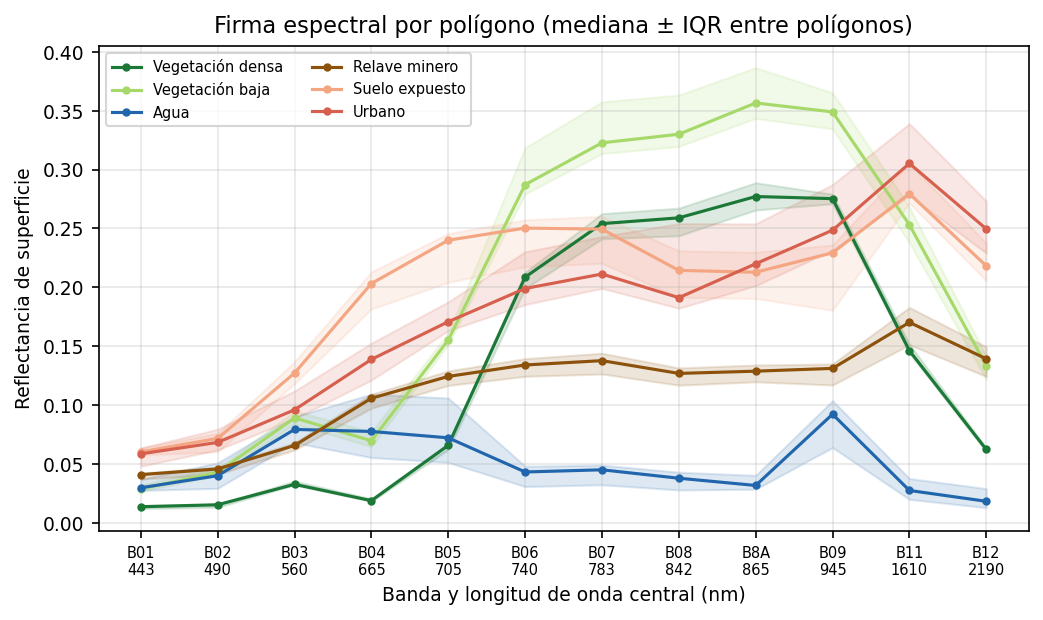
\includegraphics[width=0.85\textwidth]{figures/firmas_espectrales}
 \caption{Firma espectral por polígono: mediana e IQR entre polígonos de cada clase.}
 \label{fig:firmas}
\end{figure}

\subsection{Preprocesamiento}
Sobre el TSV se aplicaron dos transformaciones antes de entrenar:
\begin{enumerate}
 \item \textbf{Conversión a reflectancia:} los valores de las bandas se dividieron entre 10\,000.
 \item \textbf{Estandarización:} cada variable se transformó a media 0 y desviación estándar 1 con \texttt{StandardScaler}. El estandarizador se ajustó únicamente con los datos de entrenamiento y se aplicó después a los de prueba, para no filtrar información del conjunto de prueba.
\end{enumerate}
Para la pista B se construyó un dataset auxiliar con una fila por polígono: mediana de cada banda, IQR, número de píxeles e índices NDVI, NDWI, MNDWI, NDBI y BSI. Esos 17 valores (12 bandas y 5 índices) son las variables de la pista B.

\section{Metodología}

\subsection{División en entrenamiento y prueba}
Los píxeles de un mismo polígono son vecinos y casi idénticos entre sí. Si se repartieran al azar entre entrenamiento y prueba, el modelo se evaluaría con píxeles prácticamente iguales a los que ya vio y las métricas quedarían infladas \parencite{Roberts2017}. Por eso la división se hizo \textbf{por polígono}: en cada clase se eligieron al azar 4 de los polígonos originales para prueba y el resto para entrenamiento, con una semilla fija (42). La prueba son 24 polígonos originales; los polígonos añadidos en la ampliación se usan únicamente para entrenamiento (Tabla~\ref{tab:division} y Figura~\ref{fig:division}). Ningún polígono aparece en ambos conjuntos.

\begin{table}[htbp]
 \centering
 \caption{División del conjunto de datos por polígono.}
 \label{tab:division}
 \begin{tabular}{lrrrr}
  \toprule
  Clase & Polígonos entren. & Píxeles entren. & Polígonos prueba & Píxeles prueba \\
  \midrule
  Vegetación densa & 8 & 200 & 4 & 100 \\
  Vegetación baja & 8 & 200 & 4 & 100 \\
  Agua & 8 & 72 & 4 & 36 \\
  Relave minero & 8 & 200 & 4 & 100 \\
  Suelo expuesto & 13 & 325 & 4 & 100 \\
  Urbano & 8 & 72 & 4 & 36 \\
  \midrule
  Total & 53 & 1069 & 24 & 472 \\
  \bottomrule
 \end{tabular}
\end{table}


\begin{figure}[htbp]
 \centering
 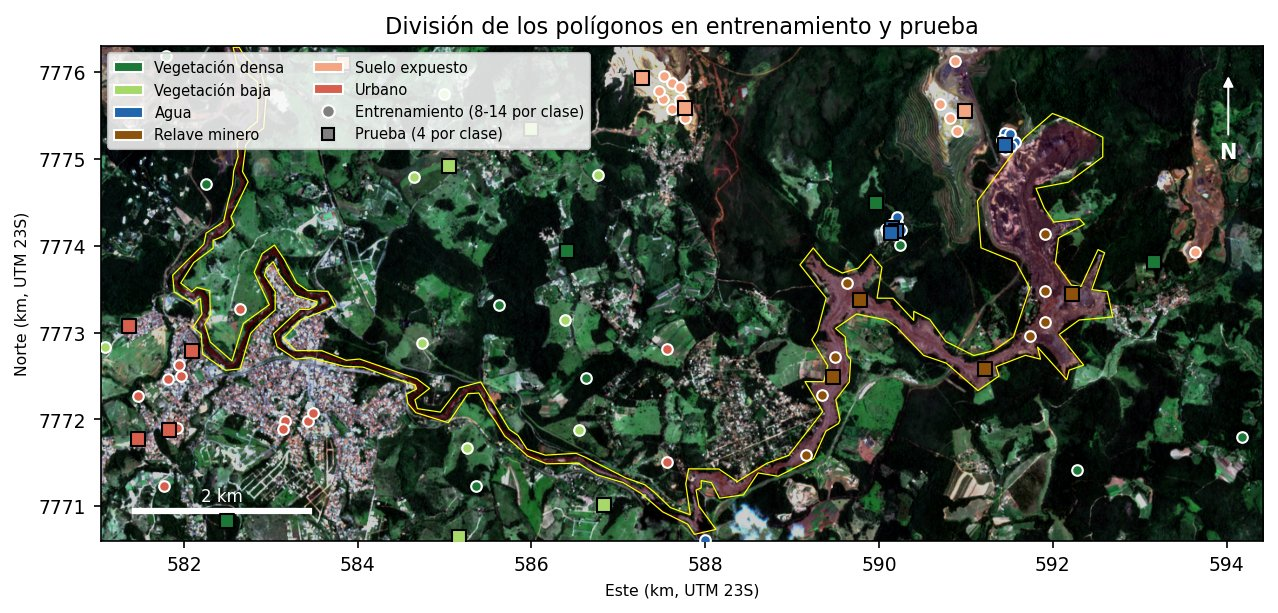
\includegraphics[width=\textwidth]{figures/division_poligonos}
 \caption{Polígonos de entrenamiento (círculos) y de prueba (cuadrados) sobre la imagen en color verdadero.}
 \label{fig:division}
\end{figure}

Este diseño mantiene el mismo conjunto de prueba para vegetación, agua, relave y urbano, pero no para suelo: se retiraron \texttt{5\_03} y \texttt{5\_11}, y la prueba de suelo pasó de \texttt{5\_03}, \texttt{5\_05}, \texttt{5\_10} y \texttt{5\_11} a \texttt{5\_04}, \texttt{5\_05}, \texttt{5\_06} y \texttt{5\_09}. Los dos polígonos retirados eran justamente los que la SVM fallaba, y se retiraron después de ver ese resultado. Una decisión así favorece a los modelos en la prueba actual, por lo que el resultado de referencia de esta fase es el de la \textbf{prueba original} (Sección~\ref{sec:referencia}). La Tabla~\ref{tab:comparacion_pareada} compara ambos entrenamientos sobre el mismo conjunto y separa el efecto de los datos del efecto del test.

Cinco polígonos añadidos quedaron por debajo de la separación mínima de la Fase~1 respecto a polígonos de prueba: \texttt{3\_13}, \texttt{3\_15} y \texttt{3\_17} a 10\,m de \texttt{3\_02}, \texttt{3\_06} y \texttt{3\_08}; \texttt{5\_16} a 40\,m de \texttt{5\_05}, y \texttt{6\_17} a 60\,m de \texttt{6\_01}. Se comprobó que entrenar sin esos cinco polígonos da la misma exactitud global en la regresión logística y en la SVM (94{,}7\,\%), así que su cercanía no infla el resultado.

\subsection{Validación cruzada y estabilidad}
Como complemento a la división única, se usó \texttt{LeaveOneGroupOut}: en cada pliegue se deja fuera un polígono completo y se entrena con los demás. Se reportan la OA y el Kappa out-of-fold, la media y el error estándar de la OA por pliegue, y un intervalo de confianza bootstrap al 95\,\% calculado remuestreando polígonos de prueba estratificados por clase.

\subsection{Modelos}
Se entrenaron los cinco modelos que pide el enunciado, más un Random Forest como complemento del árbol de decisión. La Tabla~\ref{tab:modelos} resume su configuración inicial. En los modelos que lo permiten se usaron pesos por clase (\texttt{class\_weight=balanced}) para compensar el menor número de píxeles de agua y urbano. Para el quinto modelo se eligió KNN, por ser un método no paramétrico que trabaja directamente en el espacio espectral.

\begin{table}[htbp]
 \centering
 \small
 \caption{Modelos y configuración inicial (scikit-learn). En todos, las bandas se estandarizan con \texttt{StandardScaler} ajustado solo con el entrenamiento.}
 \label{tab:modelos}
 \begin{tabularx}{\textwidth}{llX}
  \toprule
   & Modelo & Configuración inicial \\
  \midrule
  LR & Regresión logística & \texttt{max\_iter=1000}, \texttt{class\_weight=balanced} \\
  DT & Árbol de decisión & Sin límite de profundidad, criterio Gini, \texttt{class\_weight=balanced} \\
  RF & Random Forest & 300 árboles, \texttt{class\_weight=balanced} \\
  SVM & Máquina de soporte vectorial & Kernel RBF, $C=1$, $\gamma$ = \texttt{scale}, \texttt{class\_weight=balanced} \\
  ANN & Red neuronal (MLP) & Dos capas ocultas (64 y 32 neuronas), ReLU, Adam, \texttt{max\_iter=2000} \\
  KNN & K vecinos más cercanos & $k=5$, distancia euclidiana, voto uniforme \\
  \bottomrule
 \end{tabularx}
\end{table}


\subsection{Métricas}
Para cada modelo se calcularon dos niveles de evaluación:
\begin{itemize}
 \item \textbf{por píxel:} matriz de confusión, exactitud global (OA), Kappa, precisión, recall y F1;
 \item \textbf{por polígono:} voto mayoritario de las predicciones de sus píxeles, pureza (fracción de píxeles que votan por la clase mayoritaria) y acierto del polígono.
\end{itemize}
La exactitud global y el Kappa se definen como
\begin{equation}
 \mathrm{OA} = \frac{\sum_{i} n_{ii}}{N}, \qquad
 \kappa = \frac{p_o - p_e}{1 - p_e}, \qquad
 p_e = \sum_{i} \frac{n_{i+}\, n_{+i}}{N^2},
\end{equation}
donde $p_o$ es la OA, y $n_{i+}$ y $n_{+i}$ son los totales de la fila y de la columna $i$ \parencite{Cohen1960}. La precisión, el recall y el F1 se calculan por clase; el F1 macro es su promedio simple.

\section{Resultados}

\subsection{Comparación de los modelos por píxel}
Esta sección presenta primero las métricas mínimas de la fase, la exactitud global y las matrices de confusión por píxel sobre la prueba actual, y después el resultado de referencia sobre la prueba original (Sección~\ref{sec:referencia}). La Tabla~\ref{tab:metricas} y la Figura~\ref{fig:metricas} resumen las métricas de los seis modelos. En la prueba actual, la regresión logística y la SVM empatan en la mejor exactitud global (94{,}7\,\%), el mejor Kappa (0{,}935) y el mejor F1 macro (0{,}933). En la validación cruzada, la SVM obtiene la OA out-of-fold más alta (94{,}5\,\%), seguida de la regresión logística (94{,}0\,\%). El árbol de decisión individual es el modelo más débil (86{,}7\,\%), y el Random Forest lo mejora en unos cuatro puntos. La red neuronal queda en 89{,}8\,\%: su resultado es sensible a la composición de la prueba y no supera a los modelos más simples.

\begin{table}[htbp]
 \centering
 \small
\setlength{\tabcolsep}{4pt}
 \caption{Métricas sobre el conjunto de prueba (24 polígonos, 472 píxeles) y OA LOO out-of-fold $\pm$ error estándar de la OA por pliegue. En negrita, el mejor valor.}
 \label{tab:metricas}
 \begin{tabular}{llcccccc}
  \toprule
   & Modelo & OA & Kappa & Precisión & Recall & F1 & OA LOO \\
  \midrule
  LR & Regresión logística & 0{,}934 & 0{,}919 & 0{,}957 & 0{,}931 & 0{,}938 & 0{,}932 $\pm$ 0{,}026 \\
  DT & Árbol de decisión & 0{,}905 & 0{,}881 & 0{,}948 & 0{,}872 & 0{,}888 & 0{,}894 $\pm$ 0{,}034 \\
  RF & Random Forest & 0{,}939 & 0{,}924 & 0{,}957 & 0{,}934 & 0{,}941 & 0{,}917 $\pm$ 0{,}028 \\
  SVM & Máquina de soporte vectorial & 0{,}947 & 0{,}935 & 0{,}967 & 0{,}958 & 0{,}958 & 0{,}942 $\pm$ 0{,}023 \\
  ANN & Red neuronal (MLP) & \textbf{0{,}972} & \textbf{0{,}966} & \textbf{0{,}981} & \textbf{0{,}978} & \textbf{0{,}978} & 0{,}931 $\pm$ 0{,}023 \\
  KNN & K vecinos más cercanos & 0{,}939 & 0{,}924 & 0{,}957 & 0{,}940 & 0{,}945 & 0{,}923 $\pm$ 0{,}026 \\
  \bottomrule
 \end{tabular}
\end{table}


\begin{figure}[htbp]
 \centering
 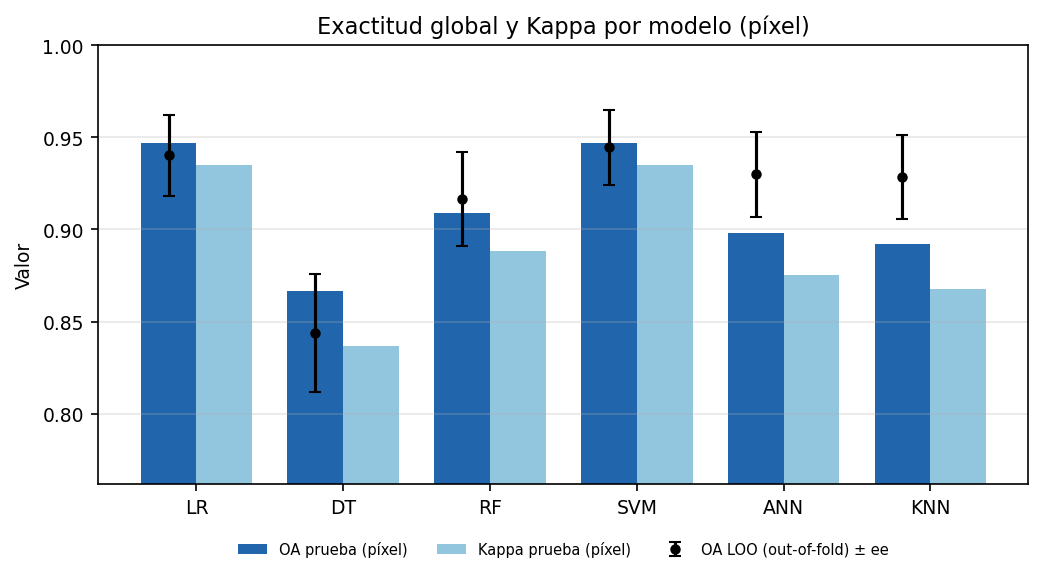
\includegraphics[width=0.85\textwidth]{figures/metricas_modelos}
 \caption{Exactitud global y Kappa sobre el conjunto de prueba, y OA out-of-fold ($\pm$ error estándar) de la validación cruzada.}
 \label{fig:metricas}
\end{figure}

\subsection{Matrices de confusión}
La Figura~\ref{fig:matrices} presenta las matrices de confusión de los seis modelos. La vegetación densa, la vegetación baja, el agua y el relave se clasifican sin errores en la regresión logística y en la SVM. El error restante está en suelo expuesto: uno de los cuatro polígonos de prueba, \texttt{5\_06}, se clasifica completo como urbano (25 píxeles). Por eso el recall de suelo es 0{,}75, la precisión del urbano es 0{,}59 y su F1 es 0{,}742.

\begin{figure}[htbp]
 \centering
 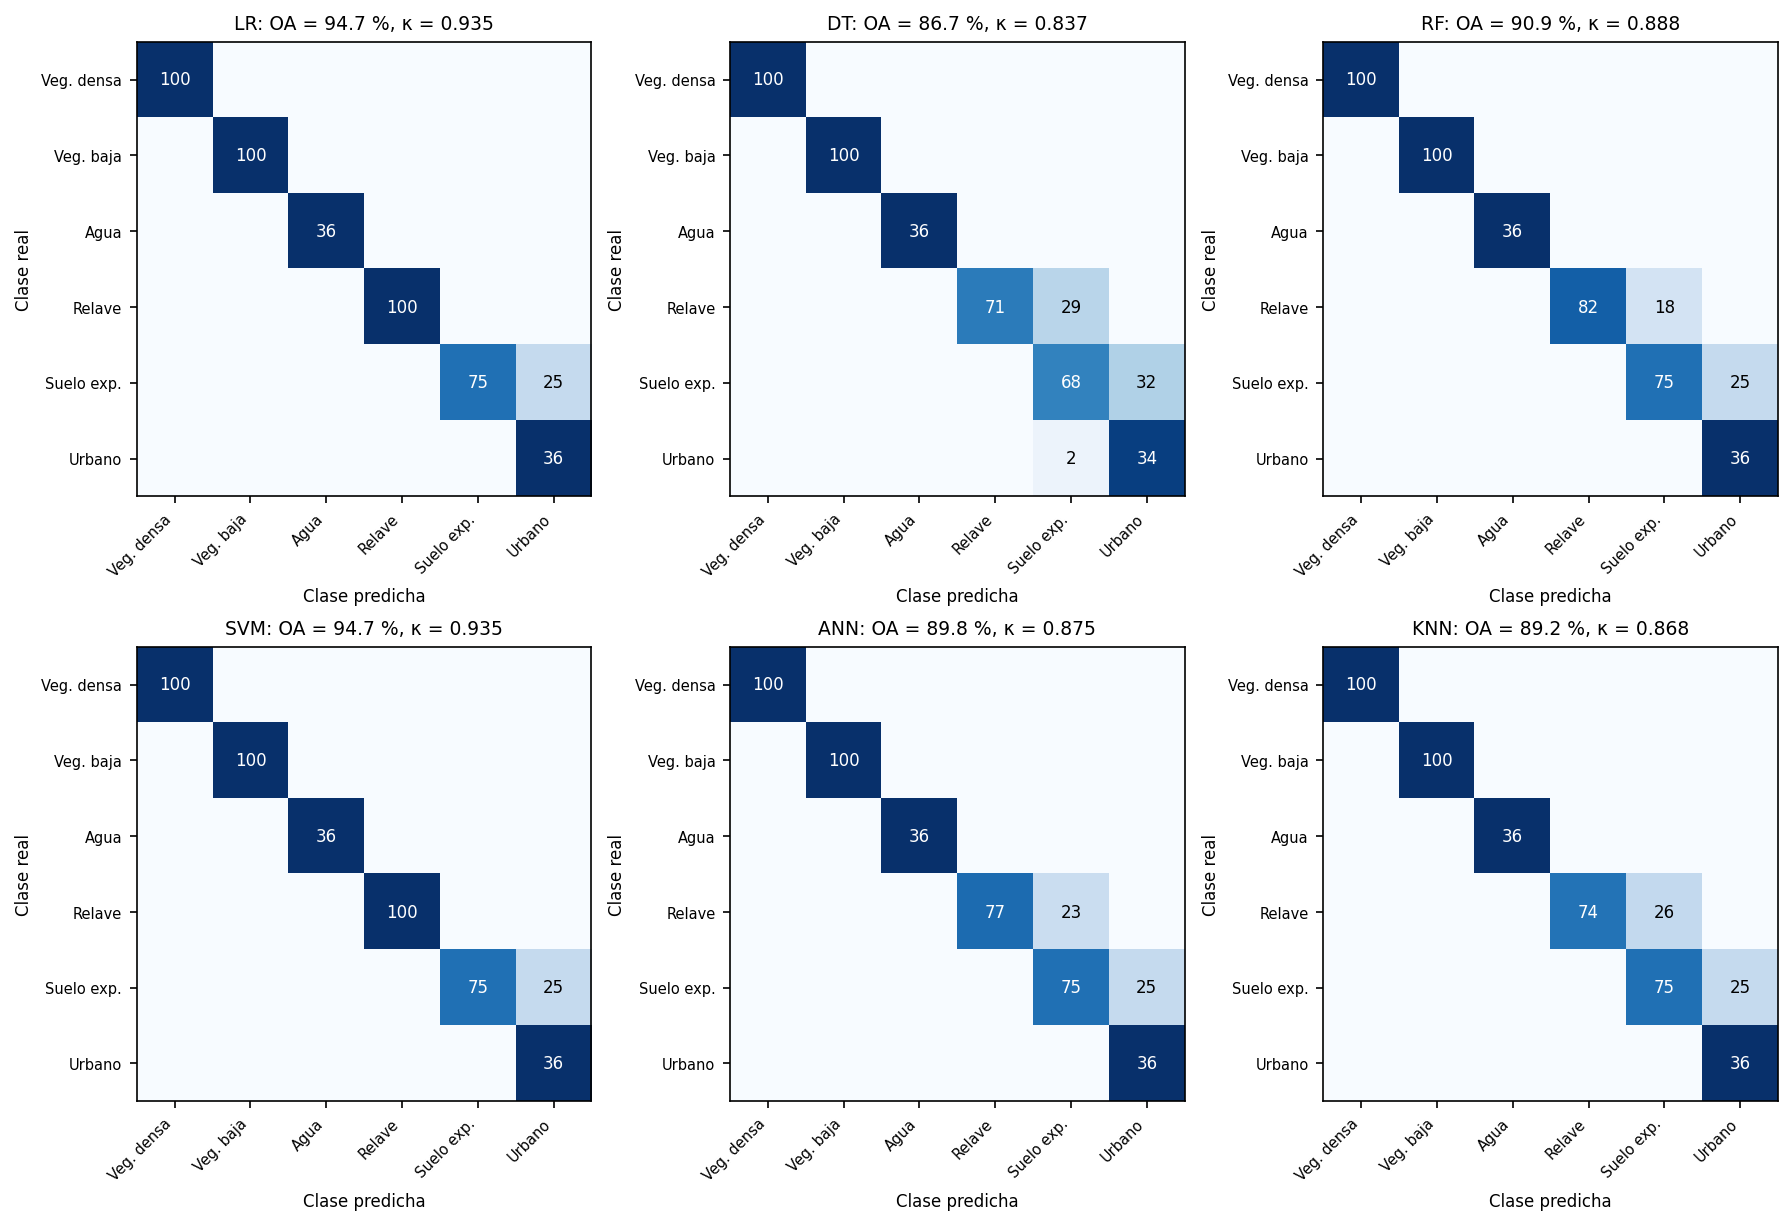
\includegraphics[width=\textwidth]{figures/matrices_confusion}
 \caption{Matrices de confusión por píxel sobre el conjunto de prueba. Los números son píxeles; el color indica la proporción respecto al total de la clase real.}
 \label{fig:matrices}
\end{figure}

La Tabla~\ref{tab:matriz_mejor} muestra la matriz de la regresión logística, que empata con la SVM en todas las métricas, y la Tabla~\ref{tab:por_clase} sus métricas por clase. La red neuronal tiene un error adicional: asigna 23 píxeles de relave a suelo, por lo que su recall de relave baja a 0{,}77 (Tabla~\ref{tab:por_clase}).

\begin{table}[htbp]
 \centering
 \small
\setlength{\tabcolsep}{3.5pt}
 \caption{Matriz de confusión del mejor modelo por píxel (Red neuronal (MLP)). Filas: clase real; columnas: clase predicha; EP: exactitud del productor; EU: exactitud del usuario.}
 \label{tab:matriz_mejor}
 \begin{tabular}{lrrrrrrrr}
  \toprule
  Real / Predicha & Veg. densa & Veg. baja & Agua & Relave & Suelo exp. & Urbano & Total & EP (\%) \\
  \midrule
  Veg. densa & 100 & 0 & 0 & 0 & 0 & 0 & 100 & 100{,}0 \\
  Veg. baja & 0 & 100 & 0 & 0 & 0 & 0 & 100 & 100{,}0 \\
  Agua & 0 & 0 & 36 & 0 & 0 & 0 & 36 & 100{,}0 \\
  Relave & 0 & 0 & 0 & 87 & 13 & 0 & 100 & 87{,}0 \\
  Suelo exp. & 0 & 0 & 0 & 0 & 100 & 0 & 100 & 100{,}0 \\
  Urbano & 0 & 0 & 0 & 0 & 0 & 36 & 36 & 100{,}0 \\
  \midrule
  Total & 100 & 100 & 36 & 87 & 113 & 36 & 472 & \\
  EU (\%) & 100{,}0 & 100{,}0 & 100{,}0 & 100{,}0 & 88{,}5 & 100{,}0 & & \\
  \bottomrule
 \end{tabular}
\end{table}


\begin{table}[htbp]
 \centering
 \caption{Precisión, recall y F1 por clase del mejor modelo por píxel (Red neuronal (MLP)).}
 \label{tab:por_clase}
 \begin{tabular}{lcccr}
  \toprule
  Clase & Precisión & Recall & F1 & Píxeles de prueba \\
  \midrule
  Vegetación densa & 1{,}000 & 1{,}000 & 1{,}000 & 100 \\
  Vegetación baja & 1{,}000 & 1{,}000 & 1{,}000 & 100 \\
  Agua & 1{,}000 & 1{,}000 & 1{,}000 & 36 \\
  Relave minero & 1{,}000 & 0{,}870 & 0{,}930 & 100 \\
  Suelo expuesto & 0{,}885 & 1{,}000 & 0{,}939 & 100 \\
  Urbano & 1{,}000 & 1{,}000 & 1{,}000 & 36 \\
  \bottomrule
 \end{tabular}
\end{table}


\subsection{Resultado de referencia: prueba original}
\label{sec:referencia}
La Tabla~\ref{tab:comparacion_pareada} compara el entrenamiento con 72 polígonos (base) y con 88 (nuevo) sobre el mismo conjunto de prueba. En la \textbf{prueba original}, definida antes de la ampliación y que incluye \texttt{5\_03} y \texttt{5\_11}, la SVM se mantiene en 0{,}894 y la regresión logística sube de 0{,}883 a 0{,}894. Este es el resultado de referencia de la fase: la ampliación apenas cambia el desempeño. En la prueba actual, la SVM sube 4{,}9 puntos y la regresión logística 0{,}4, y en los 22 polígonos comunes a ambas pruebas los dos modelos son casi perfectos. Por tanto, la diferencia entre 89{,}4\,\% y 94{,}7\,\% se debe sobre todo a la composición de la prueba de suelo, no a los datos nuevos.

\begin{table}[htbp]
 \centering
 \small
 \setlength{\tabcolsep}{4pt}
 \caption{Comparación pareada del efecto de la ampliación (OA). \emph{Original 24}: test de la versión de 72 polígonos. \emph{Nuevo 24}: test de la versión de 88. \emph{Común 22}: test original sin \texttt{5\_03} ni \texttt{5\_11}. La base del test nuevo se entrena solo con polígonos originales que no están en ese test, para evitar fuga.}
 \label{tab:comparacion_pareada}
 \begin{tabular}{lcccc}
  \toprule
  Test & Modelo & Base & Nuevo & $\Delta$ \\
  \midrule
  Original 24 & LR & 0{,}883 & 0{,}894 & $+0{,}011$ \\
  Original 24 & SVM & 0{,}894 & 0{,}894 & $0{,}000$ \\
  Nuevo 24 & LR & 0{,}943 & 0{,}947 & $+0{,}004$ \\
  Nuevo 24 & SVM & 0{,}898 & 0{,}947 & $+0{,}049$ \\
  Común 22 & LR & 0{,}988 & 1{,}000 & $+0{,}012$ \\
  Común 22 & SVM & 1{,}000 & 1{,}000 & $0{,}000$ \\
  \bottomrule
 \end{tabular}
\end{table}


\subsection{Evaluación por polígono}
La Figura~\ref{fig:matrices_pol} presenta las matrices de confusión por polígono de la pista B (medianas por polígono) y la Tabla~\ref{tab:metricas_poligono} compara las dos pistas. En la pista A, la regresión logística y la SVM aciertan 23 de los 24 polígonos de prueba (OA 0{,}958, Kappa 0{,}950); el único error es \texttt{5\_06}. En la pista B, la regresión logística y el Random Forest también alcanzan 0{,}958/0{,}950. Las diferencias entre modelos son de uno o dos polígonos, por lo que no son concluyentes.

\begin{figure}[htbp]
 \centering
 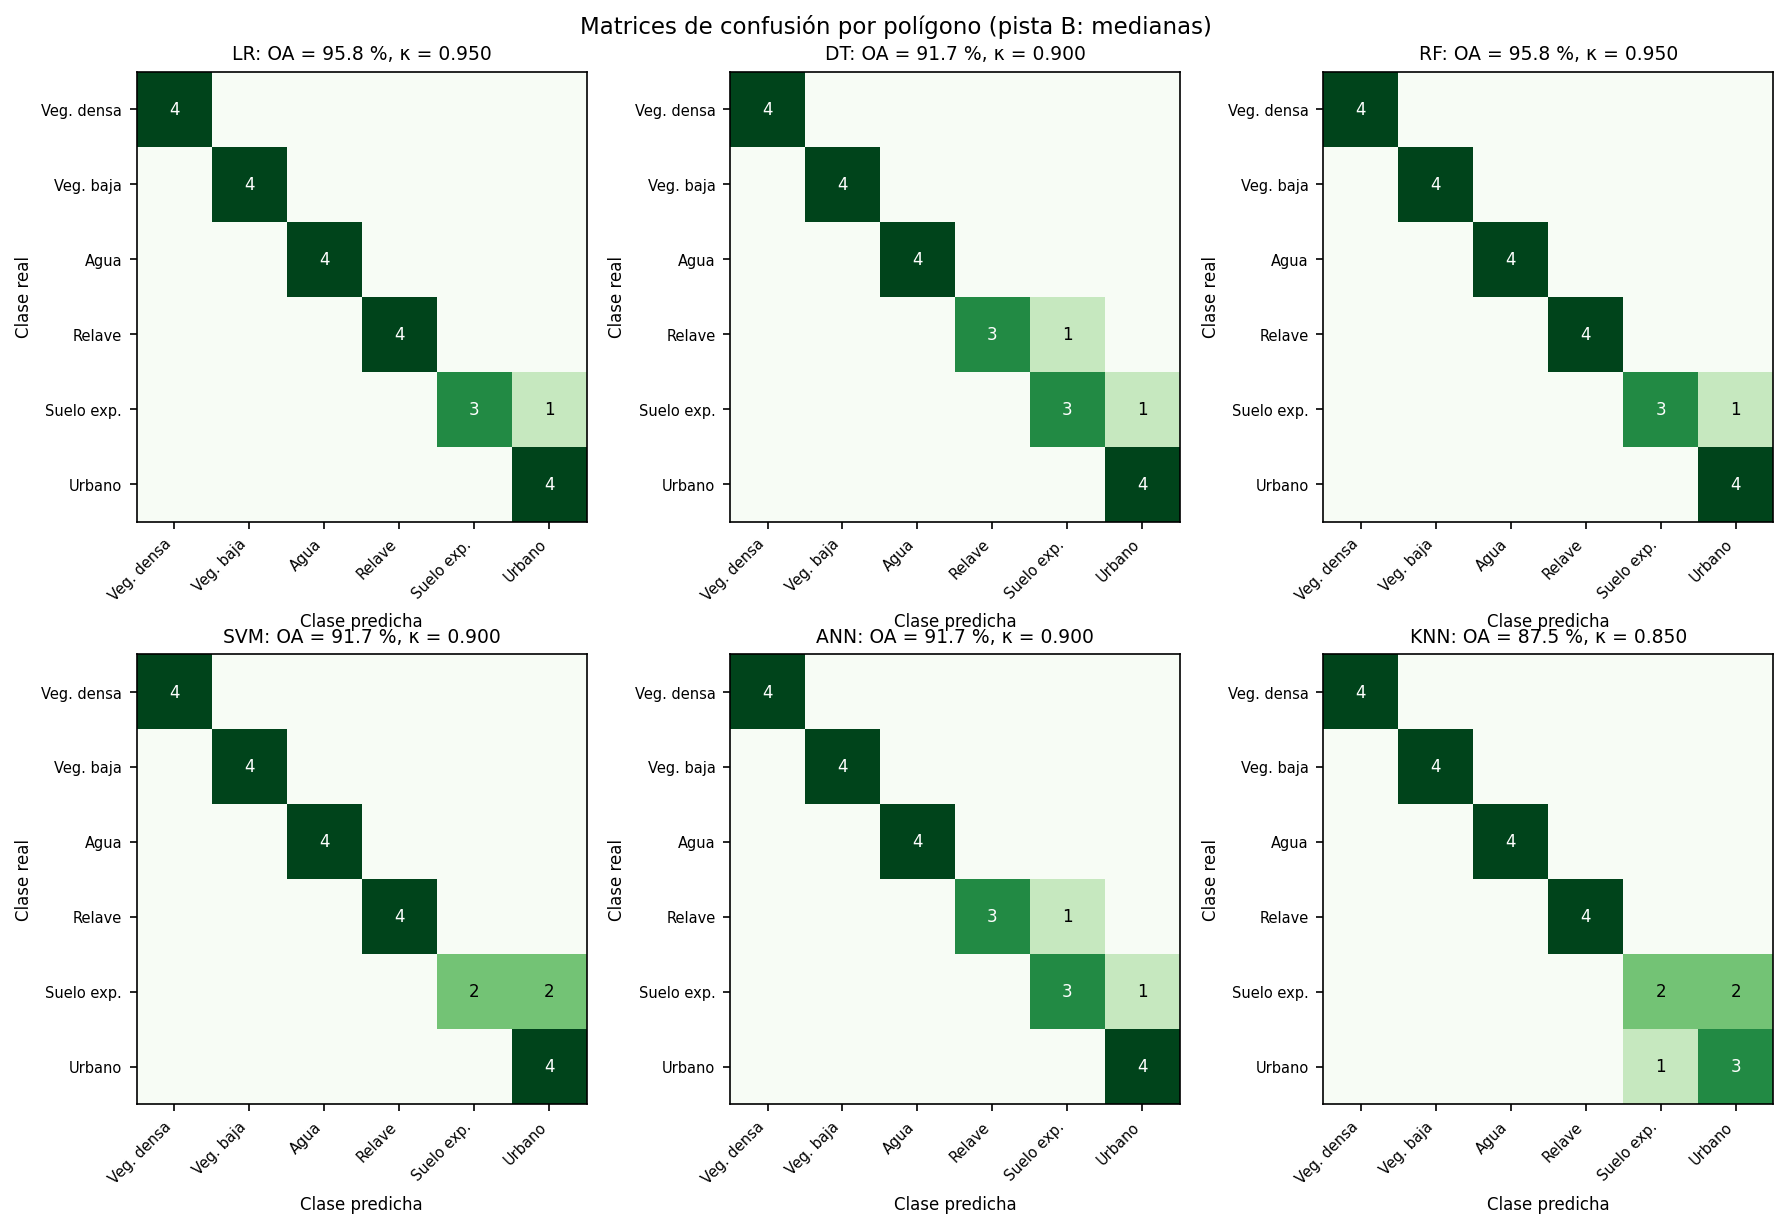
\includegraphics[width=\textwidth]{figures/matrices_confusion_poligono}
 \caption{Matrices de confusión por polígono de la pista B (medianas por polígono). Los números son polígonos.}
 \label{fig:matrices_pol}
\end{figure}

\begin{table}[htbp]
 \centering
 \small
\setlength{\tabcolsep}{3.5pt}
 \caption{Métricas por polígono (24 de prueba). Pista A: votación mayoritaria de las predicciones por píxel; pista B: mediana por polígono e índices. Las diferencias de uno o dos polígonos no son concluyentes.}
 \label{tab:metricas_poligono}
 \begin{tabular}{lccccccc}
  \toprule
  Modelo & A OA & A Kappa & A F1 & A pureza & B OA & B Kappa & B F1 \\
  \midrule
  LR & 0{,}917 & 0{,}900 & 0{,}915 & 0{,}986 & 0{,}958 & 0{,}950 & 0{,}958 \\
  DT & 0{,}875 & 0{,}850 & 0{,}875 & 0{,}987 & 0{,}958 & 0{,}950 & 0{,}958 \\
  RF & 0{,}958 & 0{,}950 & 0{,}958 & 0{,}969 & 0{,}958 & 0{,}950 & 0{,}958 \\
  SVM & 0{,}958 & 0{,}950 & 0{,}958 & 1{,}000 & 0{,}917 & 0{,}900 & 0{,}907 \\
  ANN & 1{,}000 & 1{,}000 & 1{,}000 & 0{,}978 & 0{,}958 & 0{,}950 & 0{,}958 \\
  KNN & 0{,}958 & 0{,}950 & 0{,}958 & 0{,}978 & 0{,}917 & 0{,}900 & 0{,}916 \\
  \bottomrule
 \end{tabular}
\end{table}


\begin{figure}[htbp]
 \centering
 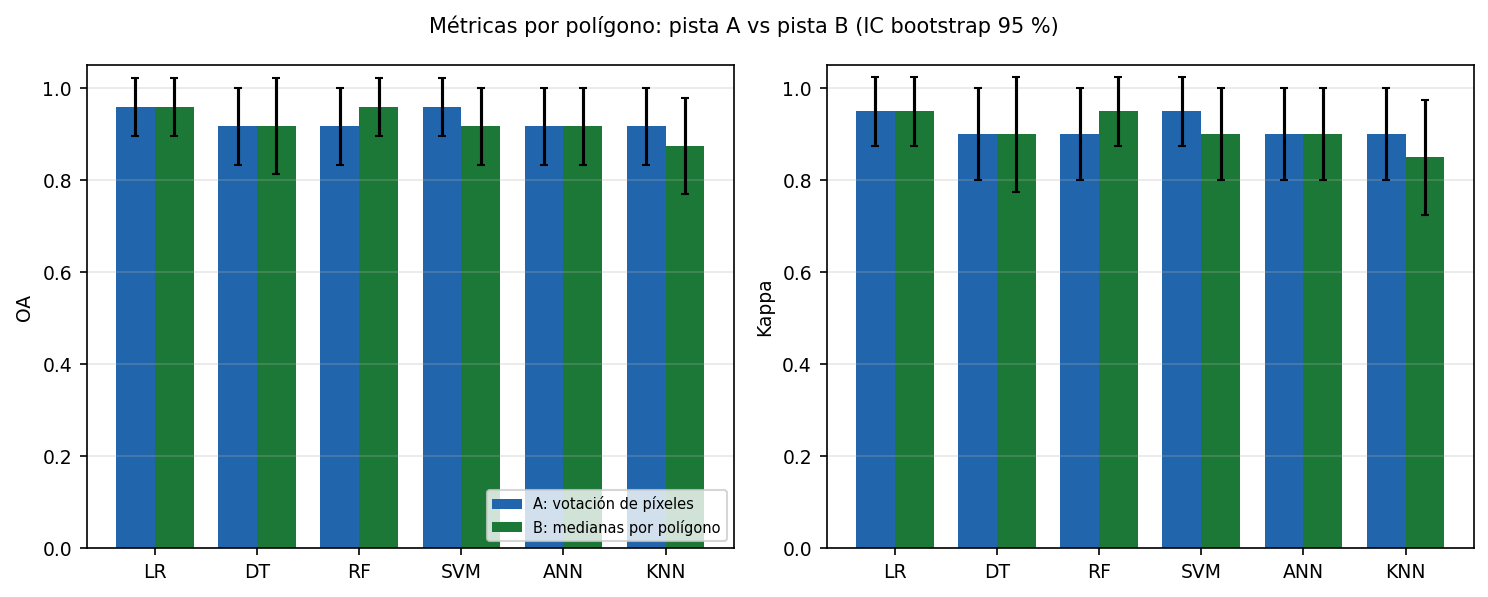
\includegraphics[width=0.95\textwidth]{figures/metricas_poligono}
 \caption{OA y Kappa por polígono de las pistas A y B, con IC bootstrap al 95\,\%.}
 \label{fig:metricas_pol}
\end{figure}

La Tabla~\ref{tab:pureza} y la Figura~\ref{fig:pureza} muestran la pureza media y el acierto medio por polígono de la pista A. La regresión logística y la SVM tienen pureza 1{,}000: todos los píxeles de cada polígono votan por una sola clase, aunque en \texttt{5\_06} la clase mayoritaria es la incorrecta.

\begin{table}[htbp]
 \centering
 \small
 \caption{Pureza media (fracción de píxeles que votan por la clase mayoritaria) y acierto medio por polígono en la pista A.}
 \label{tab:pureza}
 \begin{tabular}{lcc}
  \toprule
  Modelo & Pureza media & Acierto medio \\
  \midrule
  LR & 0{,}981 & 0{,}894 \\
  DT & 0{,}944 & 0{,}819 \\
  RF & 0{,}948 & 0{,}849 \\
  SVM & 1{,}000 & 0{,}917 \\
  ANN & 0{,}955 & 0{,}898 \\
  KNN & 0{,}975 & 0{,}850 \\
  \bottomrule
 \end{tabular}
\end{table}


\begin{figure}[htbp]
 \centering
 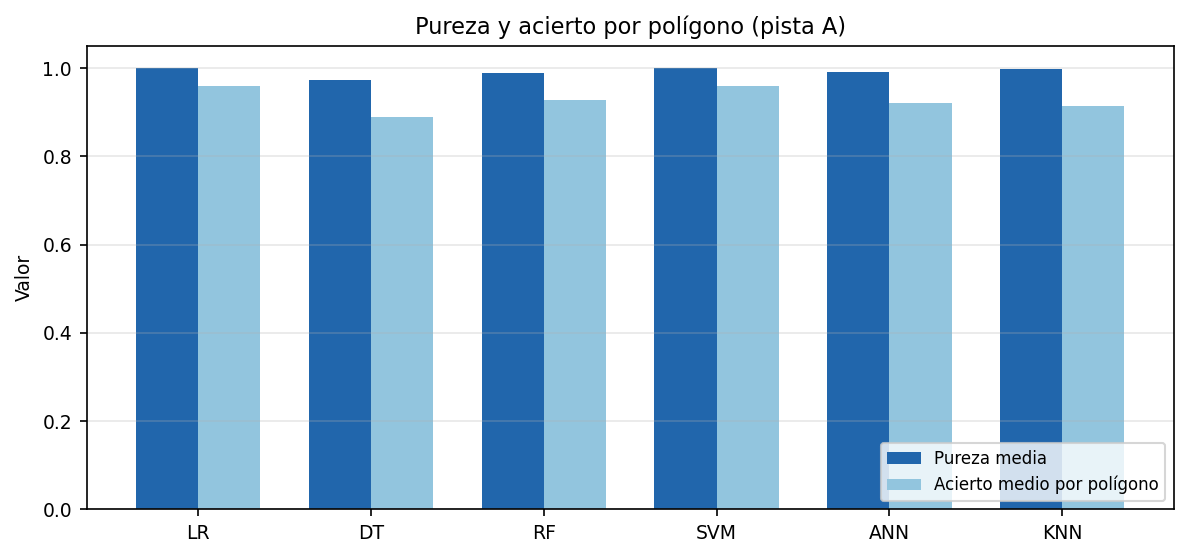
\includegraphics[width=0.85\textwidth]{figures/pureza_poligonos}
 \caption{Pureza media y acierto medio por polígono de la pista A.}
 \label{fig:pureza}
\end{figure}

\subsection{Comparación píxel vs polígono}
La Tabla~\ref{tab:pixel_vs_poligono} y la Figura~\ref{fig:pixel_vs_poligono} comparan las tres evaluaciones. Al pasar de píxel a polígono, la OA de la regresión logística sube de 0{,}947 a 0{,}958 y la de la SVM también sube de 0{,}947 a 0{,}958. La evaluación por polígono es más estable porque evita que unos pocos píxeles mezclados dominen la métrica, pero también es más gruesa: solo hay 24 polígonos de prueba.

\begin{table}[htbp]
 \centering
 \small
 \caption{Comparación de la unidad de evaluación: píxel, polígono A (votación) y polígono B (medianas).}
 \label{tab:pixel_vs_poligono}
 \begin{tabular}{lcccccc}
  \toprule
  Modelo & OA píxel & Kappa píxel & OA pol. A & Kappa pol. A & OA pol. B & Kappa pol. B \\
  \midrule
  LR & 0{,}883 & 0{,}857 & 0{,}875 & 0{,}850 & 0{,}917 & 0{,}900 \\
  DT & 0{,}788 & 0{,}741 & 0{,}875 & 0{,}850 & 0{,}875 & 0{,}850 \\
  RF & 0{,}835 & 0{,}797 & 0{,}875 & 0{,}850 & 0{,}917 & 0{,}900 \\
  SVM & 0{,}894 & 0{,}870 & 0{,}917 & 0{,}900 & 0{,}917 & 0{,}900 \\
  ANN & 0{,}871 & 0{,}841 & 0{,}917 & 0{,}900 & 0{,}875 & 0{,}850 \\
  KNN & 0{,}828 & 0{,}789 & 0{,}875 & 0{,}850 & 0{,}875 & 0{,}850 \\
  \bottomrule
 \end{tabular}
\end{table}


\begin{figure}[htbp]
 \centering
 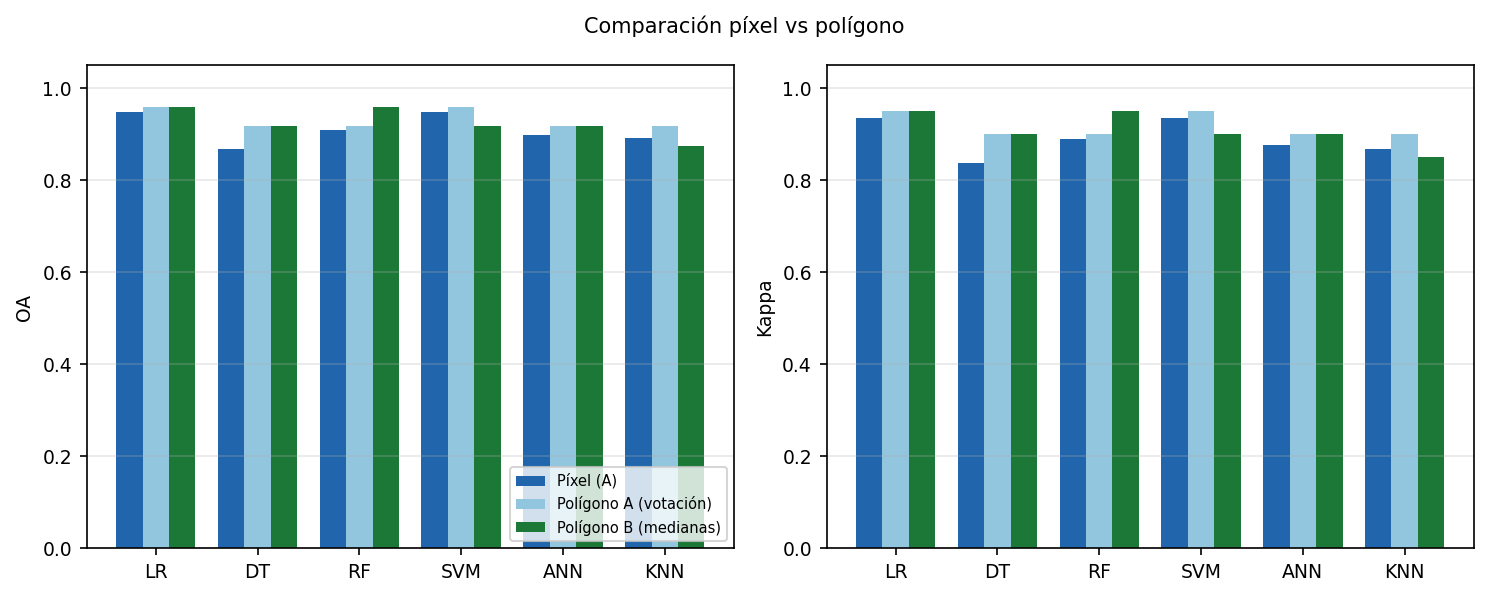
\includegraphics[width=0.95\textwidth]{figures/pixel_vs_poligono}
 \caption{OA y Kappa según la unidad de evaluación: píxel, polígono A (votación) y polígono B (medianas).}
 \label{fig:pixel_vs_poligono}
\end{figure}

\subsection{Unidad de muestreo y tamaño efectivo}
La Tabla~\ref{tab:icc} presenta la correlación intraclase (ICC) por banda y el tamaño efectivo de muestra. El ICC es 0{,}932--0{,}995 y el tamaño efectivo es 88--94, no 1640. Es decir, los píxeles de un mismo polígono aportan muy poca información independiente. Esto justifica partir y evaluar por polígono, y explica por qué añadir píxeles dentro de los polígonos existentes no equivale a añadir datos.

\begin{table}[htbp]
 \centering
 \small
 \caption{Correlación intraclase (ICC) por banda y tamaño efectivo de muestra considerando el polígono como unidad.}
 \label{tab:icc}
 \begin{tabular}{lcc}
  \toprule
  Banda & ICC & $n_{\mathrm{eff}}$ \\
  \midrule
  B01 & 0{,}993 & 72{,}5 \\
  B02 & 0{,}952 & 75{,}4 \\
  B03 & 0{,}964 & 74{,}5 \\
  B04 & 0{,}974 & 73{,}8 \\
  B05 & 0{,}980 & 73{,}4 \\
  B06 & 0{,}986 & 73{,}0 \\
  B07 & 0{,}988 & 72{,}8 \\
  B08 & 0{,}980 & 73{,}4 \\
  B8A & 0{,}992 & 72{,}5 \\
  B09 & 0{,}996 & 72{,}3 \\
  B11 & 0{,}990 & 72{,}7 \\
  B12 & 0{,}989 & 72{,}7 \\
  \bottomrule
 \end{tabular}
\end{table}


\subsection{Importancia de las variables}
La Figura~\ref{fig:importancia} muestra la importancia de las bandas en la pista A. El árbol de decisión se apoya en B8A, B12 y B02; el Random Forest reparte la importancia entre B8A, B12 y B04. La Figura~\ref{fig:importancia_pol} muestra la pista B: NDVI, NDWI y MNDWI concentran la mayor importancia, seguidas de B03, B07 y B12. Esta importancia debe leerse con cuidado: NDVI, NDWI y MNDWI son los mismos índices con los que se propusieron las etiquetas, así que su peso está inflado por construcción y no demuestra que aporten información nueva.

\begin{figure}[htbp]
 \centering
 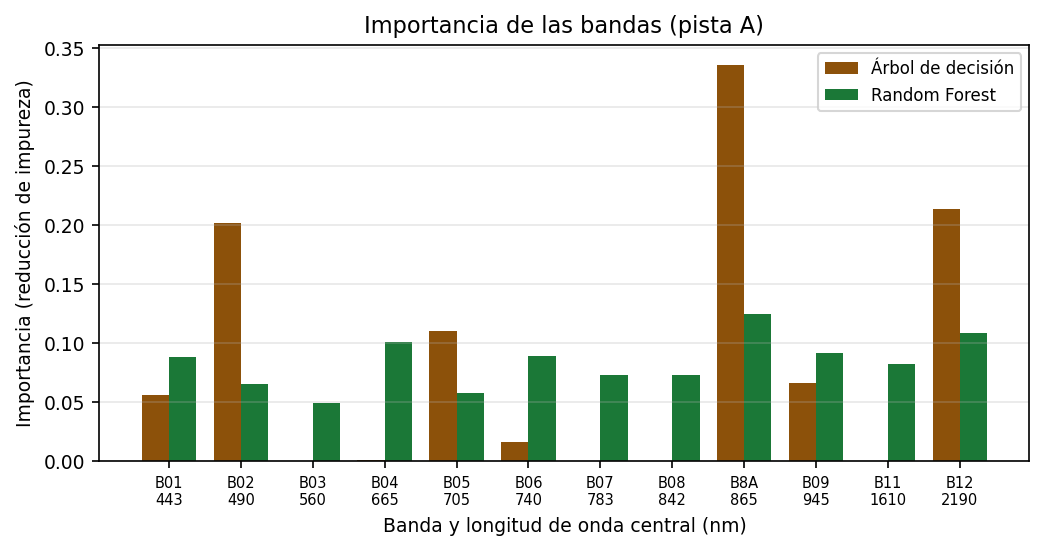
\includegraphics[width=0.85\textwidth]{figures/importancia_bandas}
 \caption{Importancia de las bandas (reducción media de la impureza de Gini) en el árbol de decisión y el Random Forest de la pista A.}
 \label{fig:importancia}
\end{figure}

\begin{figure}[htbp]
 \centering
 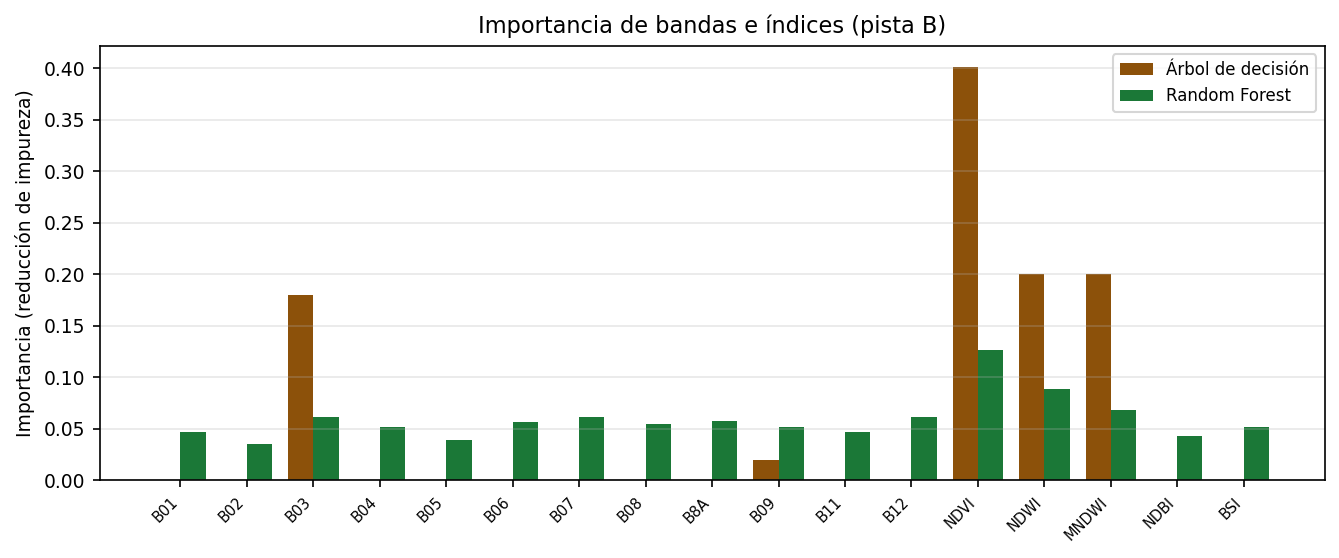
\includegraphics[width=0.95\textwidth]{figures/importancia_bandas_poligono}
 \caption{Importancia de bandas e índices en el árbol de decisión y el Random Forest de la pista B.}
 \label{fig:importancia_pol}
\end{figure}

\section{Discusión}
Los resultados indican que las doce bandas permiten separar con exactitud la vegetación, el agua y el relave. La dificultad está en suelo expuesto y urbano: sus firmas son parecidas y, a 10\,m, un polígono de suelo puede contener lotes, vías o materiales de construcción. El error de \texttt{5\_06} es consistente con esa ambigüedad: no es un píxel aislado, es un polígono completo.

La ampliación del dataset no mejoró de forma demostrable el desempeño. Se retiraron dos polígonos de suelo después de ver que la SVM los fallaba y se añadieron candidatos de suelo, agua y urbano al entrenamiento. Sobre la prueba original la SVM se mantiene en 89{,}4\,\% y la regresión logística sube 1{,}1 puntos, hasta 89{,}4\,\%. El 94{,}7\,\% de la prueba actual describe un conjunto sin los dos polígonos difíciles, no una mejora de los modelos. La red neuronal queda en 0{,}898 en la prueba actual, por debajo de los modelos más simples.

Quedan limitaciones. Las etiquetas son pseudo-etiquetas construidas con reglas espectrales y revisión visual, no verdad de campo. Cinco polígonos añadidos quedaron a 10--60\,m de polígonos de prueba, por debajo de la separación mínima de la Fase~1; aunque se comprobó que no cambian la exactitud, introducen autocorrelación espacial. Los 72 polígonos originales y los candidatos de suelo no tuvieron revisión visual individual. El test tiene solo 24 polígonos y las clases de vegetación y relave siguen con 12 polígonos cada una. Por eso las diferencias de uno o dos polígonos no deben interpretarse como superioridad definitiva.

\section{Próximos pasos}
En la Fase~3 se realizarán las siguientes tareas:
\begin{itemize}
 \item optimizar los hiperparámetros de cada modelo, por ejemplo $C$ y $\gamma$ en la SVM, la arquitectura de la red neuronal, $k$ en KNN y la profundidad del árbol, con validación cruzada agrupada por polígono;
 \item revisar visualmente los polígonos sin revisión individual (los 72 originales y los candidatos de suelo) con un criterio definido de antemano, no según los errores del modelo; añadir polígonos de suelo y urbano más puros, separados de los de prueba, y ampliar vegetación y relave;
 \item comparar los modelos optimizados con Kappa, precisión, recall y F1, y seleccionar el mejor;
 \item aplicar el modelo seleccionado a toda la imagen para obtener el GeoTIFF temático, simbolizarlo en QGIS y calcular el área de cada clase.
\end{itemize}

\printbibliography

\end{document}
